\documentclass[a4paper]{article}
\usepackage[utf8]{inputenc}
\usepackage[T1]{fontenc}
\usepackage[english,brazilian]{babel} 
\usepackage[a4paper, left=20mm, right=20mm, top=20mm, bottom=20mm]{geometry}
%\usepackage{indentfirst} %uncomment this for paragraph indentation
\usepackage{xspace}
\usepackage{graphicx}
\usepackage[hyperfootnotes=false,bookmarks]{hyperref}
\usepackage[perpage,bottom]{footmisc}
\usepackage{caption}
\usepackage{subcaption}
\usepackage[nottoc]{tocbibind}
\captionsetup[figure]{position=above,labelsep=period}
\captionsetup[table]{position=above,labelsep=period}
\setlength{\parskip}{\baselineskip}
\setlength\parindent{0pt} % comment this for paragraph indentation
\title{DESENVOLVIMENTO E IMPLANTAÇÃO DE SISTEMA \textit{WEB} PARA GERENCIAMENTO DA BIBLIOTECA DO CURSO EXATO}
\begin{document}

%%%%%%%%%%%%%%%%%%%%%%%%%%%%%%%%%%%%%%%%%%%%
%%% Cabeçalho baseado no padrão do Exato %%%
%%%%%%%%%%%%%%%%%%%%%%%%%%%%%%%%%%%%%%%%%%%%
\begin{minipage}[t|]{14mm}
\includegraphics[width=2cm]{img/logo-unicamp.eps}
\end{minipage}
\hfill
\begin{minipage}[tl]{120mm}
\begin{center}
{\bf \sc Projeto Final de Graduação}\\
{\bf \sc Instituto de Computação} \\
{\bf \sc Universidade Estadual de Campinas} \\
\end{center}
\end{minipage}
\hfill
\begin{minipage}[c]{25mm}
\thispagestyle{empty}
\hspace{-0.5cm}
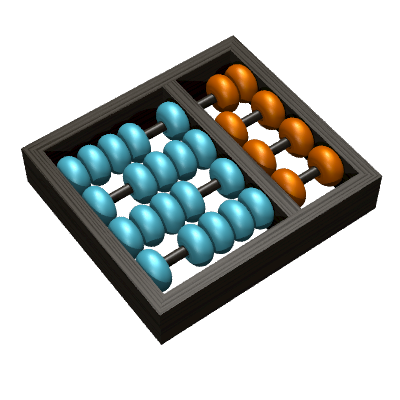
\includegraphics[width=25mm]{img/logo-ic.png}
\end{minipage}
\vfill\vfill
\begin{center}
\Huge{\textbf{DESENVOLVIMENTO E IMPLANTAÇÃO DE SISTEMA\textit{WEB} PARA GERENCIAMENTO DA BIBLIOTECA DO CURSO EXATO}}
\vfill\vfill
\huge{Davi Kooji Uezono\\Gustavo Fumio Oyakawa}
\vfill
\Large{Supervisores: Fábio Luiz Usberti e Christiane Neme Campos}
\vfill\vfill
\Large{Dezembro de 2015}
\end{center}
\vfill

\pagebreak
\pagenumbering{roman}
\begin{abstract}
\normalsize
Esta monografia descreve um projeto final de graduação para o curso de Engenharia de Computação pelo Instituto de Computação (IC) da Unicamp. Foi elaborado um sistema \textit{web} para administração da biblioteca do Curso Exato, um projeto de extensão comunitária da Unicamp. Tomou-se o sistema de gerenciamento de conteúdo \textit{Drupal} como base para a aplicação, que incluiu, além das facilidades esperadas para um sistema de biblioteca virtual, funcionalidades sociais como troca de mensagens entre usuários e perfil pessoal com espaço para preferências literárias. Seguiu-se a metodologia \textit{Scrum} para desenvolvimento ágil, com a motivação de manter o envolvimento das partes interessadas no projeto e garantir entregas contínuas de um \textit{software} funcional.
\end{abstract}

\selectlanguage{english} 
\begin{abstract}
\normalsize
This paper describes a final graduation project for the Computer Engineering major under Unicamp's Institute of Computing (IC). We developed a loan library management web system for Curso Exato, one of Unicamp's educational outreach projects. The \textit{Drupal} content management system was used as foundation for this application, that included not only the required functionalities for maintaining the library, but also social features like private messaging and literary preferences sharing through personal profiles. The Scrum methodology for agile development was followed, with the intention to retain the stakeholders' involvement and ensure continuous delivery of functioning software.
\end{abstract}
\selectlanguage{brazilian} 

\pagebreak
\tableofcontents{}

%%%%%%%%%%%%%%%%%%%%%%%%%%%%
%% INTRODUÇÃO E OBJETIVOS %%
%%%%%%%%%%%%%%%%%%%%%%%%%%%%
\pagebreak
\clearpage
\pagenumbering{arabic}
\setcounter{page}{1}
\section{Introdução e objetivos}

O Curso Exato é um projeto de extensão comunitária da Preac (Pró-Reitoria de Extensão e Assuntos Comunitários) da Unicamp, que "tem por objetivo contribuir para o desenvolvimento de alunos da rede pública de ensino. Para isso, o projeto oferece aulas nas áreas de Física, Matemática, Português e Química, visando à consolidação e ao aprofundamento dos conhecimentos adquiridos no Ensino Médio" \ \cite{cursoexato}.

Aumentar o contato dos jovens com os livros é um grande obstáculo enfrentado hoje pelo Curso Exato. Por esta razão, em 2014 foi iniciado um projeto para a criação de uma biblioteca, a fim de incentivar o hábito da leitura. Para tanto, os membros do Curso Exato organizaram uma campanha de arrecadação de livros por meio de doações, e hoje conta com mais de cem títulos. Neste contexto, o desafio passou a ser catalogar os livros e organizar o processo de empréstimo, possibilitando a circulação dos livros.

Com o intuito de aproximar os alunos dos livros e aproveitando-se do contexto atual de inclusão tecnológica, propõe-se neste projeto a criação de um sistema \textit{web} de gerenciamento de biblioteca para os alunos, professores voluntários e coordenadores do Curso Exato. A criação deste sistema para consulta ao acervo, reservas e empréstimos tem o intuito de ampliar a capacidade de funcionamento da biblioteca, tornando-a acessível para todos os alunos pelo meio digital, já que a frequência deles ao espaço físico da biblioteca é impossibilitada por questões de logística (os livros ficam trancados em armários em um prédio distante daquele onde ocorrem as aulas. Além disso, o prédio da biblioteca não possui uma estrutura que permita a criação de uma recepção, na qual trabalharia o membro do projeto responsável pelo empréstimo dos livros. Desta forma, este precisa necessariamente ser feito à distância e, portanto, a criação deste site se mostrou uma solução adequada).

O principal objetivo deste projeto é desenvolver, na plataforma \textit{Drupal}\footnote{Um CMS e \textit{framework} (coleção de \textit{software} que fornece uma estrutura básica para o desenvolvimento de sistemas) de código aberto.}, um sistema \textit{web} de gerenciamento de biblioteca que atenda às necessidades do Curso Exato. Tal sistema deve seguir os padrões de código da comunidade \textit{Drupal}, para que possa ser estendido e utilizado por terceiros. Esta plataforma foi escolhida por ser de familiaridade dos desenvolvedores e dos membros do Curso Exato, e também por ser personalizável, extensível, de fácil manutenção e de baixo custo aos futuros administradores da biblioteca.

Com este sistema, os usuários da biblioteca poderão consultar os exemplares disponíveis no acervo, ver características das obras catalogadas (como nome do autor, data de publicação e sinopse), reservar um livro para empréstimo e renovar o item emprestado. Também será possível ao usuário entrar em contato com a administração para sugerir novos títulos para aquisição ou enviar comentários sobre o novo sistema. Haverá uma página de ajuda que estará disponível ao usuário a um clique, a partir de qualquer página do portal. Ainda, cada usuário da biblioteca terá um perfil pessoal na plataforma, a partir do qual será possível atribuir uma nota de uma a cinco estrelas para um livro, além de poder escrever uma resenha sobre a obra.

A meta final é não apenas prover os requisitos básicos de um sistema de biblioteca virtual, mas também engajar os usuários dentro da própria plataforma, de forma a estimular a leitura por meio dela.

As próximas seções deste texto estão estruturadas em: \textit{Metodologia de trabalho}, em que são detalhados os procedimentos seguidos pelos desenvolvedores, o escopo do projeto e suas premissas iniciais; \textit{Ciclos de desenvolvimento}, em que são descritas as atividades realizadas e os desafios encontrados durante três períodos produtivos; \textit{Resultados}, em que há uma discussão sobre o que foi produzido, o que não foi possível fazer e a aceitação do sistema pelos usuários finais; e \textit{Conclusão}, em que há um levantamento dos aspectos positivos e negativos a partir da experiência de criação do projeto pelos alunos desenvolvedores.

Ao longo do texto adota-se a seguinte notação para se referir aos principais atores envolvidos no projeto:
\begin{itemize}
\item \textit{Aluno desenvolvedor} ou \textit{graduando}: Davi ou Gustavo, os alunos de graduação responsáveis pelo desenvolvimento do sistema;
\item \textit{Supervisor}: Professor Fábio Usberti ou Professora Christiane Campos, do Instituto de Computação (IC) da Unicamp, responsáveis por orientar os alunos desenvolvedores na elaboração deste texto e na realização do projeto;
\item \textit{Responsável pela biblioteca}: membro do Curso Exato que supervisiona o funcionamento da biblioteca;
\item \textit{Professor voluntário}: membro do Curso Exato que leciona em nome do projeto de extensão;
\item \textit{Aluno (do Curso Exato)}: público-alvo do projeto de extensão.
\end{itemize}

%%%%%%%%%%%%%%%%
%% MONOGRAFIA %%
%%%%%%%%%%%%%%%%

\section{Metodologia de trabalho}
O processo de desenvolvimento do \textit{software} se iniciou por meio de metodologias ágeis \cite{manifesto}, uma vez que ambos os desenvolvedores estão habituados a tal prática. Neste modelo de desenvolvimento, afirma-se que, apesar de processos, ferramentas, documentação abrangente, contratos e planos estritos serem importantes, os indivíduos (\textit{stakeholders}) e suas interações, a entrega de um \textit{software} em funcionamento, a colaboração com o consumidor e a rápida resposta às mudanças são também relevantes.

Como o \textit{Scrum} \cite{scrum} é uma das metodologias ágeis mais utilizadas em Engenharia de \textit{Software}, ele foi escolhido para nortear os desenvolvedores. Nele, ciclos curtos de desenvolvimento (\textit{sprints}) são precedidos por um ou dois dias de reuniões para refinar a lista de tarefas e para discutir a solução técnica para o problema a ser resolvido no período. Esses ciclos são concluídos com um dia de reunião, na qual é feita uma retrospectiva para avaliar o processo de desenvolvimento recém-concluído, além de realizar uma demonstração funcional do sistema para os principais \textit{stakeholders} - neste caso, a coordenadora geral do Curso Exato e os supervisores.

Cada \textit{sprint} teve duração aproximada de quatro semanas, demarcadas pelos dias de entrega de conteúdo escrito aos supervisores do projeto. A Tabela \ref{cronograma} contém os períodos e as datas originalmente propostos.

\begin{table}[hc]
\centering
\caption{Cronograma de atividades.\label{cronograma}}
\begin{tabular}{ll}
\hline
03/08 a 04/09 & Primeiro ciclo de desenvolvimento \\
04/09 & Primeira entrega parcial da monografia \\
08/09 a 02/10 & Segundo ciclo de desenvolvimento \\
02/10 & Segunda entrega parcial da monografia \\
05/10 a 06/11 & Terceiro ciclo de desenvolvimento e validação do sistema com os usuários \\
06/11 & Terceira entrega parcial da monografia \\
06/11 a 18/12 & Melhorias finais e tradução\\
01/12 & Entrega da monografia para os professores supervisores\\
15/12 & Entrega da monografia para o Instituto de Computação\\
\hline
\end{tabular}
\end{table}

Os escopos para cada ciclo de desenvolvimento estão descritos como se segue:

\begin{itemize}
\item Primeiro ciclo: extração de requisitos e codificação da infraestrutura básica do sistema; criação de páginas de publicações do acervo, de usuários e de busca, além da principal; definições dos aspectos visuais do sistema; e desenvolvimento de ferramentas que facilitem o cadastro de publicações no acervo.
\item Segundo ciclo: codificação das interações entre usuários e publicações; métodos para reserva, empréstimo, devolução e avaliação de publicações; controle de permissões entre diferentes tipos de usuários do sistema - anônimos (não autenticados), alunos, professores voluntários e administradores.
\item Terceiro ciclo: funcionalidades sociais, implantação e validação do sistema.
\end{itemize}

A distribuição de tarefas entre os alunos desenvolvedores ocorreu em reuniões de planejamento, no início de cada ciclo de desenvolvimento. Tal fato se justifica pela grande quantidade de tecnologias envolvidas no projeto, o que inviabilizou uma divisão precisa das tarefas de cada ciclo com grande antecedência. Por este motivo, cada aluno desenvolvedor se comprometeu a realizar atividades associadas a papéis exercidos por desenvolvedores de \textit{software} em times ágeis\footnote{Grupos de desenvolvedores que atuam seguindo os princípios de metodologia ágil.}, que são:
\begin{itemize}
\item Arquiteto: responsável pelo projeto da infraestrutura do servidor \textit{web}, no qual o sistema estará hospedado.
\item Engenheiro de requisitos: responsável pela extração dos requisitos funcionais e não funcionais do sistema, por meio do contato frequente com os \textit{stakeholders}.
\item Desenvolvedor \textit{front-end}: responsável pelo \textit{design} da interface do sistema com o usuário (UI) e pela experiência do usuário (UX).
\item Desenvolvedor \textit{back-end}: responsável pela programação das funcionalidades previstas do sistema, conforme especificado pelo documento de requisitos.
\end{itemize}

O aluno Davi assumiu os papéis de Arquiteto e Desenvolvedor \textit{back-end}, enquanto o aluno Gustavo assumiu os papéis de Engenheiro de requisitos e Desenvolvedor \textit{front-end}.

Ao longo do primeiro ciclo de desenvolvimento, foi elaborado um documento contendo as premissas a respeito do desenvolvimento do projeto, visando proteger o escopo inicial e garantir o cumprimento do acordo por todas as partes envolvidas (desenvolvedores e voluntários do Curso Exato). Conforme a necessidade, foram sendo adicionados novos itens a este documento. Estes estão descritos nas seções seguintes.

\subsection{Aspectos técnicos}\label{ssec:tech}

O projeto foi desenvolvido e implementado com o \textit{software} \textit{Drupal}, na versão 7 do seu núcleo. Todos os recursos de sistema requeridos pelo trabalho são os mesmos descritos na página de requisitos do \textit{Drupal} \cite{requirements} e caberá aos interessados possuir uma infraestrutura capaz de suportar a aplicação, isentando os alunos desenvolvedores da responsabilidade da implantação do sistema. A manutenção do sistema será realizada pelos desenvolvedores até o término de 2015, incluindo um treinamento para garantir continuamente a segurança da plataforma.

Por motivos de usabilidade e segurança, foi imposto um sistema de permissões tal que diferentes classes de usuários tenham acesso apenas às funcionalidades que lhes são relevantes. Ficam definidas as seguintes classes de usuários aceitos pelo sistema:
\begin{itemize}
\item Usuário anônimo ou visitante: usuário não autenticado no sistema. Não possui, necessariamente, ligação com o Curso Exato;
\item Usuário comum ou aluno: aluno do Curso Exato cadastrado e autenticado;
\item Usuário bibliotecário: membro do Curso Exato com permissão de gerenciar a biblioteca (realizar empréstimos, registrar multas, etc.), cadastrado e autenticado;
\item Usuário superadministrador ou desenvolvedor: cadastrado e autenticado, responsável pela manutenção do sistema. Possui permissões máximas no sistema.
\end{itemize}
Ao longo deste texto, o termo \emph{usuário autenticado} é utilizado para se referir às três últimas classes de usuário e, \emph{administrador}, para se referir às duas últimas.

Considerou-se inicialmente desenvolver uma integração com o \textit{Facebook} para casos de uso simples, tais como autenticação única e recomendação de publicações a outros usuários. No entanto, a Interface de Programação de Aplicações (API) disponibilizada pelo \textit{Facebook} passa por alterações a cada dois anos, podendo comprometer a integração com o sistema aqui desenvolvido. Os  desenvolvedores do projeto haviam planejado estudar a viabilidade desta integração no início do terceiro ciclo, como mencionado anteriormente, contudo, conhecendo o funcionamento da rede social citada, decidiu-se que esta integração não seria criada, ficando como uma proposta de melhoria para o futuro.

O sistema foi projetado para ter um \textit{design} adaptável, com alguns elementos responsivos (elementos se reposicionam e se redimensionam conforme a mudança da largura da tela), exceto nas páginas administrativas. Os desenvolvedores garantem o suporte ao sistema para que este funcione corretamente nas últimas versões estáveis dos principais navegadores \textit{desktop} e \textit{mobile} (\textit{Mozilla Firefox}, \textit{Google Chrome}, \textit{Internet Explorer}, \textit{Safari} e \textit{Android Browser}). O navegador \textit{IE Mobile} não terá garantia de suporte por utilizar tecnologias mais antigas em relação aos padrões mais modernos da internet atual. Por isso, eventuais problemas de desempenho ou usabilidade podem ocorrer nestes navegadores, não sendo recomendado o seu uso.

\subsection{Aspectos relacionados à Biblioteconomia}

A identificação única de livros é uma questão consideravelmente discutida na Biblioteconomia. Neste projeto são utilizados dois tipos de identificação para cada livro: o \textit{número de chamada}, para a classificação de um livro enquanto \textit{publicação} ou \textit{obra} (entidade referente às informações contidas no livro), e o \textit{código de tombo}, para a classificação enquanto \textit{exemplar} ou \textit{cópia} de uma publicação (entidade referente a cada impressão do livro). Ambas as formas de identificação estão presentes em grande parte das bibliotecas de instituições consagradas, como universidades, e para o número de chamada especificamente existem padrões utilizados internacionalmente, como a Classificação Decimal de \textit{Dewey} \cite{dewey} e a Codificação de \textit{Cutter} \cite{cutter}. Contudo, devido à opção dos membros do Curso Exato por um código menos complexo, porém suficiente para os fins pretendidos, optou-se por não utilizar um padrão internacional. 

A principal função do número de chamada é a identificação única da publicação, utilizada para fins organizacionais do acervo da biblioteca. Este número pode ser repetido, caso os dois livros sejam exemplares da mesma publicação. O conjunto de características que definem a unicidade de uma publicação, bem como a composição desta codificação estão especificados nos próximos tópicos. O código de tombo, por sua vez, é utilizado para a identificação única do exemplar. A partir dele o bibliotecário é capaz de ter conhecimento da publicação à qual o exemplar pertence e o seu \textit{status} (disponível, reservado, emprestado, em atraso ou extraviado), além da identificação do usuário com o qual livro se encontra (se for o caso).

No contexto do Curso Exato, a unicidade de uma publicação é definida a partir do conjunto de atributos a seguir: título da obra, nome do autor, editora, ano de publicação, edição e volume. Isto significa que, no ato de cadastro, o sistema valida se existe alguma obra registrada no acervo cujos seis atributos-chave sejam os mesmos da publicação sendo cadastrada. Caso nenhuma seja encontrada, o sistema considera que a publicação é nova no acervo, atribui a ela um novo número de chamada e registra-a.

O número de chamada é formado por uma sequência de seis caracteres, dividida em três partes. A primeira parte contém duas letras, uma maiúscula e outra minúscula, indicando as duas primeiras letras do sobrenome do autor da obra. Havendo mais de um autor, toma-se apenas o primeiro autor cadastrado como referência. A segunda parte contém três dígitos e, a terceira, uma letra minúscula. Esta corresponde à primeira letra do título da obra (ainda que este comece com um artigo - ver Seção \ref{sssec:improvements}). Já os três dígitos da segunda parte são determinados da seguinte forma: dada a combinação de três letras (nome do autor e nome da obra), a primeira incidência recebe o valor 001 e a reincidência da combinação é autoincrementada (002 e assim por diante).

Em contrapartida, exemplares podem ser registrados no acervo sem que seus identificadores (códigos de tombo) contenham referências diretas às obras as quais pertencem. Espera-se que no momento do cadastro do exemplar já se conheça o número de chamada da publicação a qual ele se refere - portanto existindo uma página para ela -, para que seja possível realizar uma referência cruzada entre os dois. Mais especificamente: cada página de publicação contém uma lista de códigos de tombo dos seus exemplares disponíveis no acervo, e as páginas de exemplar contém referências para as páginas das publicações correspondentes. O código de tombo de cada exemplar é o número que o \textit{Drupal} utiliza para identificar cada conteúdo criado nesta plataforma.

Ambos os identificadores são gerados automaticamente para os livros novos que forem inseridos no sistema da biblioteca e um módulo criado no \textit{Drupal} implementa esta funcionalidade. Apesar do número de chamada gerado neste padrão só apresentar explicitamente o título da obra e do nome do autor, ele é capaz de distinguir uma obra de outra por meio dos dígitos.

Em uma biblioteca moderna, cada exemplar recebe um código de barras para automatizar o empréstimo. No escopo deste projeto isto não foi necessário, pois a quantidade de exemplares em comparação a uma biblioteca tradicional é pequena.

Como os alunos do Curso Exato não têm acesso direto ao espaço físico da biblioteca, eles dependem de um mediador (membro do Exato) responsável por retirar os livros mediante a escolha prévia dos alunos por meio do sistema \textit{on-line}.  Nesse contexto, de forma a automatizar o fluxo de empréstimo dos livros, estabeleceu-se a funcionalidade de “solicitação de reserva” do livro, permitindo ao aluno cadastrado com uma conta de usuário autenticada a escolha da obra desejada ao navegar no site. Os administradores da biblioteca são notificados desta intenção de empréstimo e deverão levar os respectivos exemplares para a sala de aula. O bibliotecário é capaz de acessar uma tela administrativa no sistema com o histórico das solicitações dos alunos e com botões para efetivar o empréstimo ou cancelar o pedido.

\section{Ciclos de desenvolvimento}
\subsection{Primeiro ciclo de desenvolvimento}

O primeiro ciclo de desenvolvimento foi iniciado com uma reunião com a principal responsável pela biblioteca do Curso Exato. Nesta reunião, foram coletadas as histórias de usuário, foi feita a validação dos requisitos do sistema e a aprovação dos escopos gerais de cada ciclo de desenvolvimento. Após este passo, realizou-se o detalhamento das tarefas a serem feitas durante o mês e suas estimativas de tempo e complexidade, com o auxílio da ferramenta \textit{Trello}\footnote{Ferramenta de gerenciamento de projetos voltado para metodologias ágeis.} \cite{trello}. Por meio desta, os alunos desenvolvedores puderam monitorar o andamento das tarefas e notificar um ao outro sobre seus progressos e eventuais dificuldades ao longo de todo o projeto.

Optou-se por hospedar uma versão de desenvolvimento do sistema na \textit{Acquia} \cite{acquia}, plataforma para computação em nuvem especializada em \textit{Drupal}. Por meio dela, ambos os desenvolvedores puderam trabalhar paralelamente na construção do sistema e apresentar uma versão funcional deste aos principais interessados - alunos e voluntários do Curso Exato, bem como supervisores deste projeto - sem a necessidade de um encontro presencial.

A seguir, são descritas as atividades realizadas durante o primeiro ciclo de desenvolvimento.

\subsubsection{Criação da página de uma publicação}

Devido à importância desta entidade no sistema, a primeira tarefa assumida foi a definição de uma publicação como um tipo de conteúdo \textit{Drupal} (página com campos fixos). Foi definido que esta página deve exibir aos usuários as seguintes informações sobre uma obra: título, foto da capa do livro, autor, ano de publicação, categoria (Luso-brasileira, Estrangeira, Infanto-juvenil ou Outros), avaliação dos usuários, resumo, editora, estado (onde a obra foi publicada), volume, coleção, edição, tradutor e número de chamada. As sete primeiras são impressas na tela assim que está é carregada; as demais ficam ocultas e são expandidas apenas se o usuário clicar na opção ‘Ver Detalhes’. Foi adicionado o botão ‘Reservar Livro’, cujo comportamento foi programado durante  o segundo ciclo de desenvolvimento (ver Seção {\ref{sssec:stransaction}}).

Há ainda os seguintes campos editáveis pelos bibliotecários, inacessíveis aos usuários não administradores: tema (Aventura, Clássico, Romance e Suspense), indicador de recomendação (variável binária representando se uma obra deve ser exibida na seção de obras recomendadas - ver Seção \ref{sssec:srecommended}) e a lista de identificadores dos exemplares da publicação na biblioteca

A disposição dos elementos na página pode ser observada nas Figuras \ref{colapsed} e \ref{expanded}.

\begin{figure}
\begin{subfigure}{.5\textwidth}
  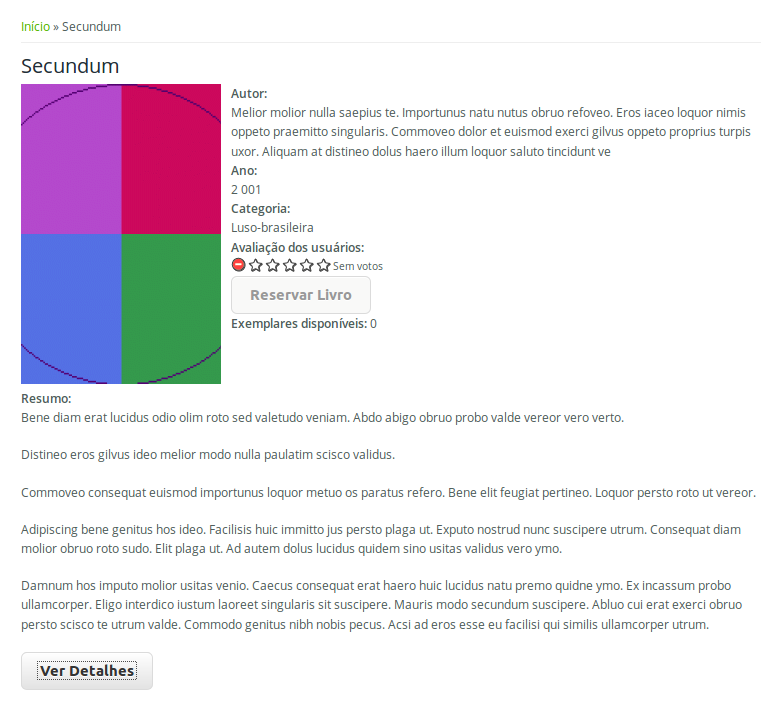
\includegraphics[width=90mm]{img/publication-colapsed.png}
  \caption{Informações adicionais ocultas.\label{colapsed}}
\end{subfigure}%
\begin{subfigure}{.4\textwidth}
  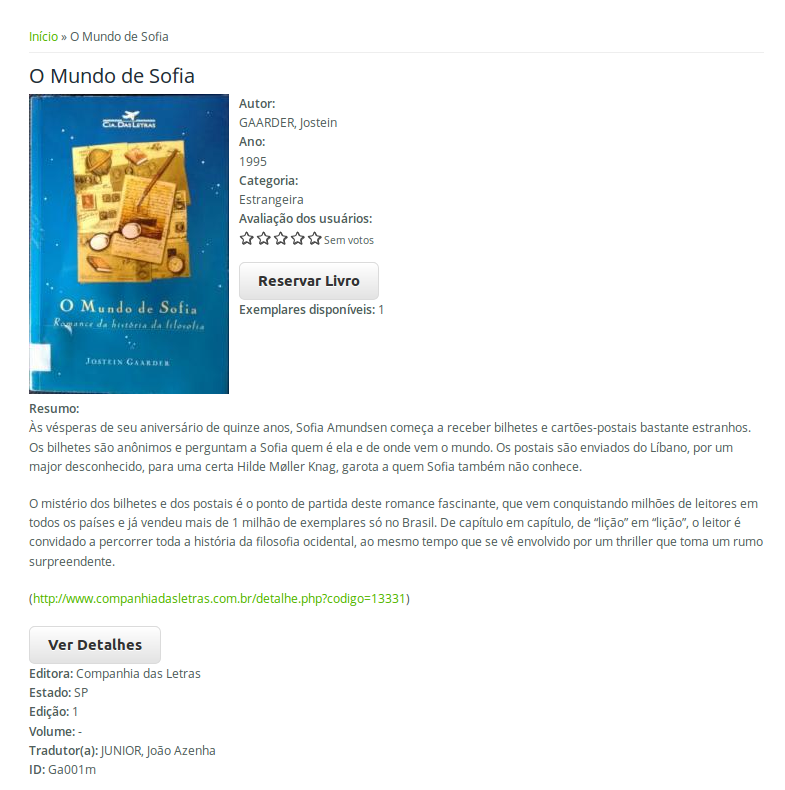
\includegraphics[width=90mm]{img/publication-expanded.png}
  \caption{Informações adicionais expandidas.\label{expanded}}
\end{subfigure}
\caption{Página de uma publicação.\label{fig:publication}}
\end{figure}


\subsubsection{Criação da página de um exemplar}

Uma segunda entidade importante é o exemplar. Esta define as múltiplas cópias de uma mesma publicação existente na biblioteca, contendo os seguintes campos: código de tombo, identificador da página da publicação a qual pertence, estado (Disponível, Reservado, Emprestado, Em atraso ou Extraviado), última data de empréstimo e última data de devolução.

No cadastro, o \textit{Drupal} cria páginas para representar cada exemplar; contudo, por serem utilizadas apenas para gerenciamento da biblioteca, decidiu-se não torná-las visíveis a usuários anônimos e alunos. Supõe-se que estes têm interesse em visualizar as páginas das publicações, e não das suas cópias.

Nota-se que os últimos quatro campos, apesar de serem declarados ainda no primeiro ciclo de desenvolvimento, passaram a ser utilizados apenas no segundo, quando começaram a ser implementadas as transações de exemplares (ver Seção \ref{sssec:stransaction}).

\subsubsection{Desenvolvimento do formulário de cadastro}

No formulário de criação de cadastro são exigidas as seguintes informações do usuário anônimo: nome completo, endereço de e-mail, ano de ingresso (no Curso Exato), endereço e telefone.

Foi habilitada a funcionalidade do \textit{Drupal} que exige a aprovação do cadastro pelos administradores para que o usuário anônimo ganhe acesso ao sistema, sendo eles notificados por e-mail quando um novo cadastro é criado. A Figura \ref{cadastro} mostra como esta seção é exibida ao usuário anônimo.

\begin{figure}[pbth!]
\centering
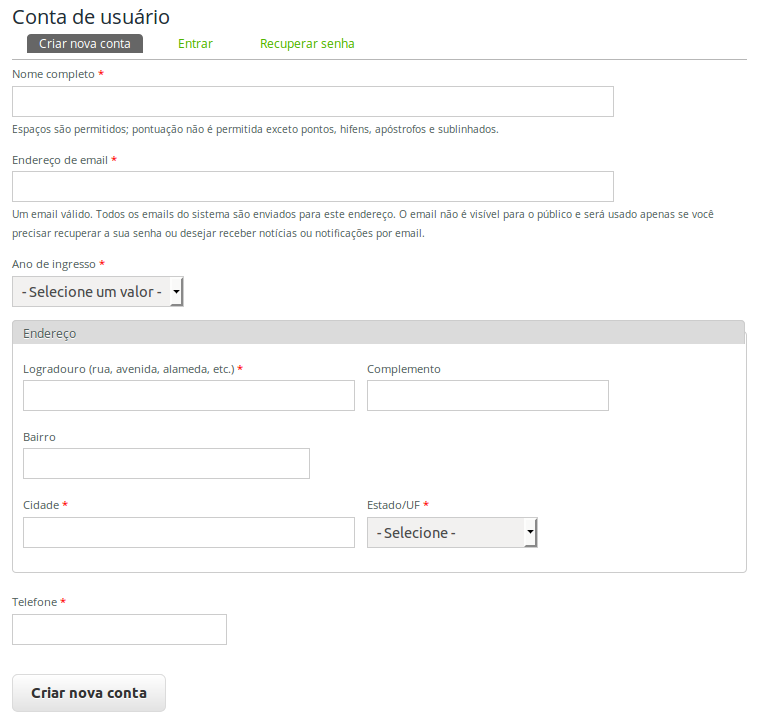
\includegraphics[width=140mm]{img/newuser.png}
\caption{Formulário de cadastro.\label{cadastro}}
\end{figure}

\subsubsection{Criação da página de um usuário}

Nesta tarefa, foi elaborada a página pessoal (ou perfil) do usuário. Nela, são exibidas nome completo, foto, ano de ingresso, autor predileto, categoria preferida e tema preferido.

Posteriormente, foi adicionado o campo “Livro de cabeceira”, no qual o usuário pode preencher com o título de sua obra predileta, sem que ela precise constar do acervo. Este campo foi adicionado com o intuito de incentivar o envolvimento dos alunos com a biblioteca e com a leitura, ao permitir maior interação e participação entre eles. Porém, foi necessário um tempo não planejado de discussão com os administradores da biblioteca para que se decidisse como o campo seria exibido. A Figura \ref{userpage} mostra o resultado final.

\begin{figure}[pbth!]
\centering
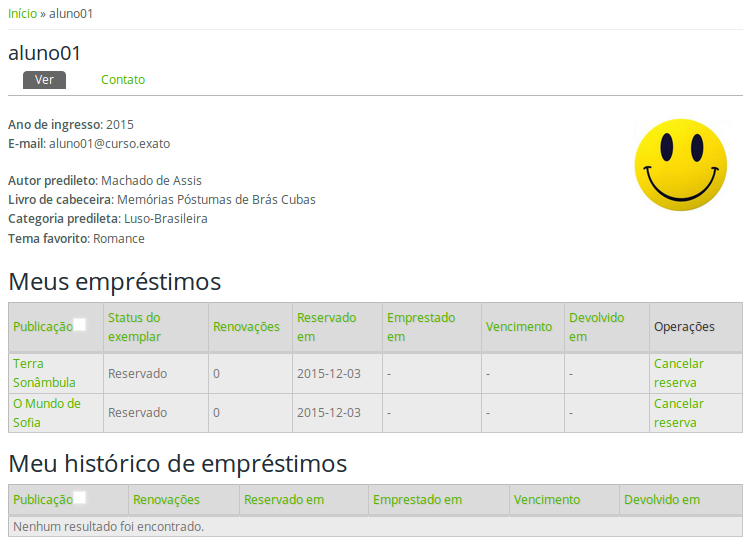
\includegraphics[width=140mm]{img/userpage.png}
\caption{Página de usuário.\label{userpage}}
\end{figure}

Ainda com o intuito de tornar a biblioteca uma plataforma mais sociável e interativa para os alunos, adicionou-se uma funcionalidade de envio de mensagens privadas entre os usuários do sistema. Para tanto, foi instalado um módulo da comunidade \textit{Drupal} chamado \textit{Privatemsg}, que já cria e habilita tal mecanismo, aproveitando os recursos de usuário e autenticação que o mesmo já oferece. Para a segurança da comunidade do Curso Exato, as mensagens podem passar por um processo de auditoria quando necessário, sendo este papel conferido apenas a um usuário específico.

Uma vez que este módulo permite o acesso às conversas de todos os usuários do sistema por um administrador, será pedido aos usuários que concordem com a política de privacidade do site para que as funcionalidades do \textit{Privatemsg} lhe estejam disponíveis. Portanto, para usar o bate-papo do site é preciso haver uma concordância dos usuários com a política de privacidade adotada pelo Curso Exato.

A Figura \ref{privatemsg} ilustra uma conversa entre dois usuários no módulo \textit{Privatemsg} e a Figura \ref{pvtmsg-config} exibe a opção de configuração na conta do usuário que possiblita a escolha pela ativação ou não de tal funcionalidade. O link nesta figura abre uma página contendo uma descrição detalhada da política de privacidade, a ser definida pelos membros do Curso Exato.

\begin{figure}[pbth!]
\centering
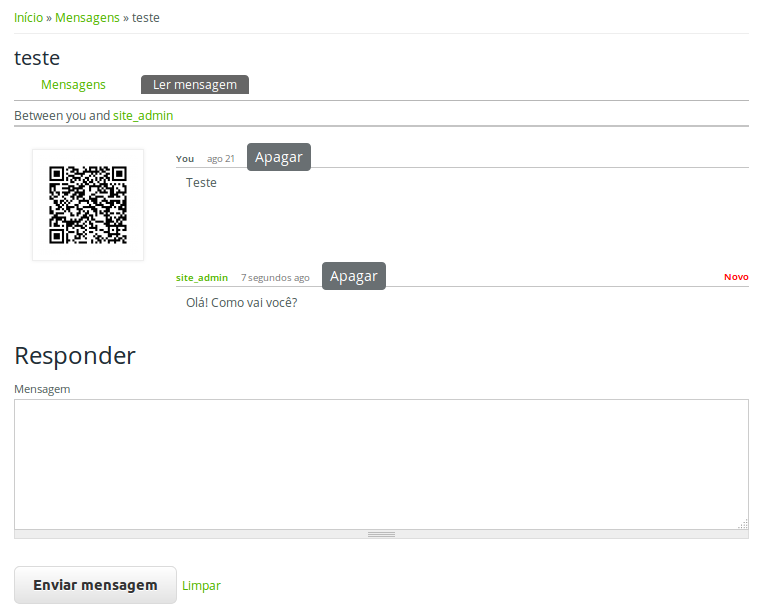
\includegraphics[width=120mm]{img/privatemsg.png}
\caption{Conversa entre dois usuários utilizando as mensagens privadas.\label{privatemsg}}
\end{figure}

\begin{figure}[pbth!]
\centering
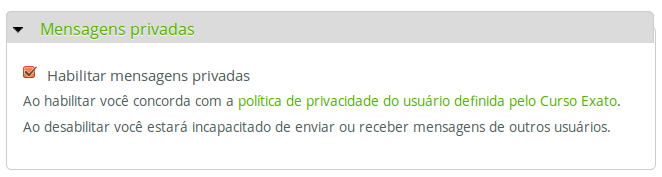
\includegraphics[width=120mm]{img/privatemsg-config.png}
\caption{Opção para o usuário ativar ou não a funcionalidade.\label{pvtmsg-config}}
\end{figure}


\subsubsection{Desenvolvimento de páginas de busca}

Foram criadas páginas de busca por publicações e por usuários, utilizando a funcionalidade \textit{view} do \textit{Drupal}, que executa consultas no banco de dados e imprime o resultado na tela de forma personalizada pelo programador. A consulta pode ser fixa ou conter parâmetros (filtros). 

No caso da página de busca por publicações, os filtros que aparecem inicialmente são apenas título e autor. O usuário pode clicar em um botão de “Busca Avançada” para exibir campos adicionais, como o ano de publicação, ou para alterar a ordenação por autor ou por título; ou ainda, alterar a ordem de exibição dos resultados - alfabética ou alfabética reversa. As Figuras \ref{simple} e \ref{advanced} ilustram as páginas de busca por publicações utilizando filtros simples ou avançados.

\begin{figure}
\begin{subfigure}{.5\textwidth}
  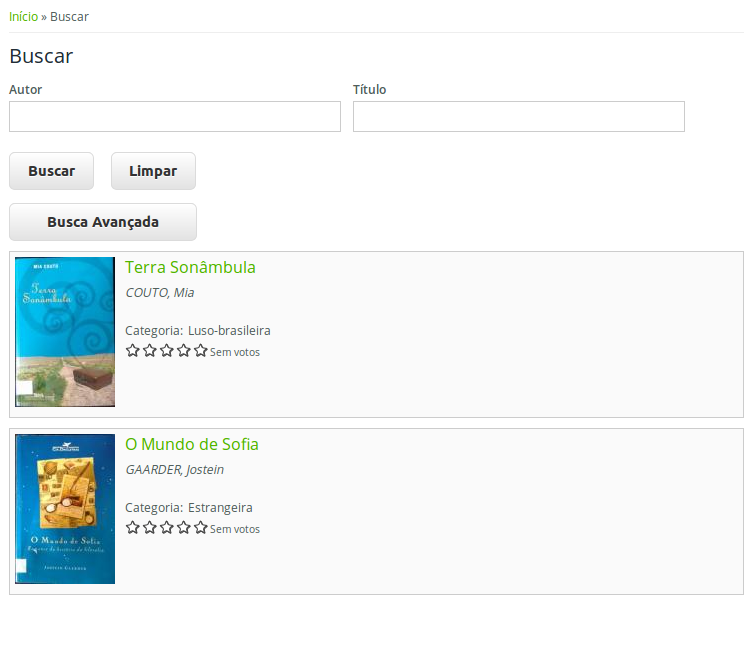
\includegraphics[width=90mm]{img/browse-simple.png}
  \caption{Filtros simples.}
  \label{simple}
\end{subfigure}%
\begin{subfigure}{.5\textwidth}
  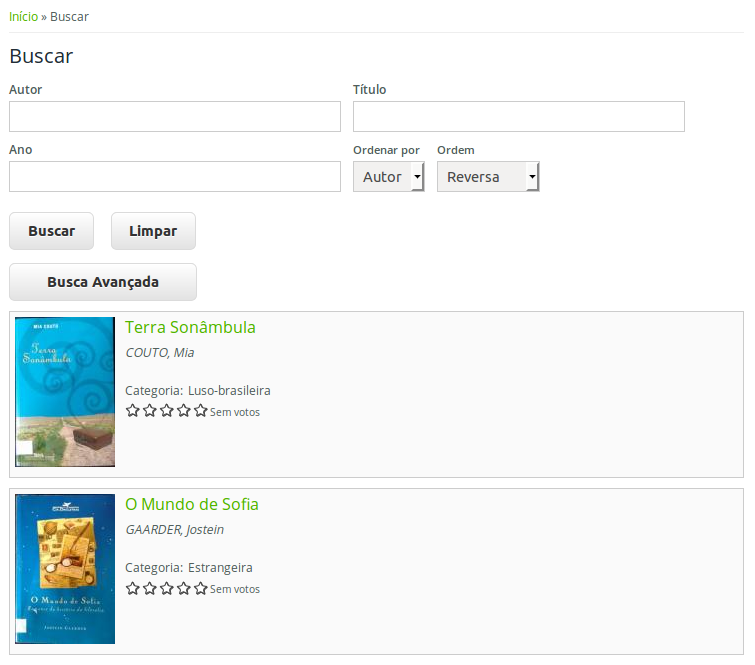
\includegraphics[width=90mm]{img/browse-advanced.png}
  \caption{Filtros avançados.}
  \label{advanced}
\end{subfigure}
\caption{Página de busca por publicações}
\label{fig:publication-search}
\end{figure}

Além disso, um pequeno formulário foi adicionado à barra lateral direita da página inicial do site para simplificar a pesquisa por publicações. Nele, o usuário pode digitar o título e/ou o nome de um autor para a pesquisa no acervo e, ao clicar no botão “Buscar”, ele será redirecionado para a página de resultados da busca, conforme a Figura \ref{browse-sidebar}.

\begin{figure}[pbth!]
\centering
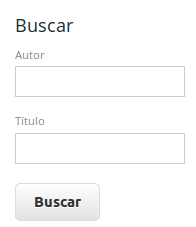
\includegraphics[width=30mm]{img/browse-sidebar.png}
\caption{Formulário de busca por publicações na barra lateral.\label{browse-sidebar}}
\end{figure}

Já no caso da página de busca por usuários, os filtros são o nome do usuário, o autor predileto, a categoria preferida e o livro de cabeceira. A Figura \ref{users} ilustra a página de busca por usuários.

\begin{figure}[pbth!]
\centering
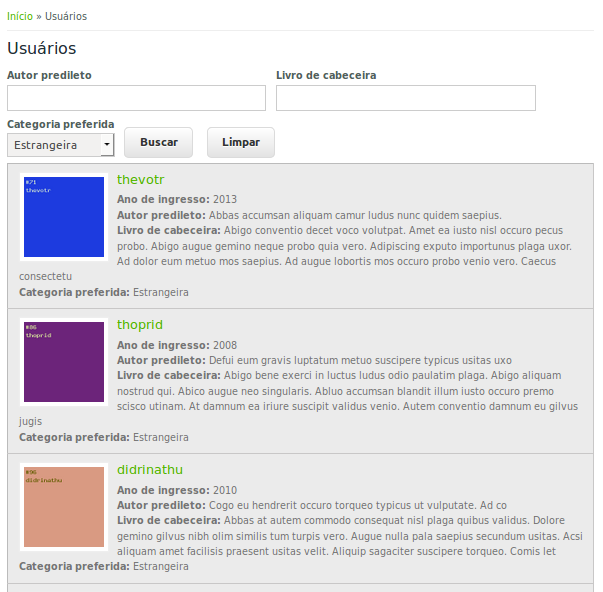
\includegraphics[width=120mm]{img/users.png}
\caption{Página de busca por usuários.\label{users}}
\end{figure}


\subsubsection{Criação da página inicial e aplicação da identidade visual do Curso Exato}

Considerou-se melhor postergar a criação da página inicial do sistema para quando houvesse uma quantidade mínima de elementos para ser exibida. A página principal foi diagramada após o encerramento das tarefas anteriores, seguindo esboço elaborado durante as reuniões iniciais de coleta de histórias de usuário.

O tema \textit{Business Responsive} foi escolhido (dentre outros disponíveis gratuitamente na comunidade \textit{Drupal}) com os administradores da biblioteca para ser a base para a elaboração dos aspectos visuais do sistema. Conforme recomendação da comunidade \textit{Drupal} e havendo permissão dos criadores do tema original, foi desenvolvido um subtema baseado no \textit{Business Responsive}, no qual foram realizadas alterações para que o sistema tivesse uma identidade visual semelhante àquela do Curso Exato.

Foi incluído também um carrossel - elemento de destaque da página com rotação de imagens - no qual serão exibidos conteúdos relevantes para os usuários, como: obras adquiridas recentemente, livros recomendados e eventos do Curso Exato. Sua inclusão se deu pela instalação do módulo \textit{Nivo Slider} (também disponível na comunidade \textit{Drupal}).

A Figura \ref{home} ilustra a página inicial para um usuário autenticado. Foi incluída uma imagem provisória para demonstração do funcionamento do carrossel.

\begin{figure}[pbth!]
\centering
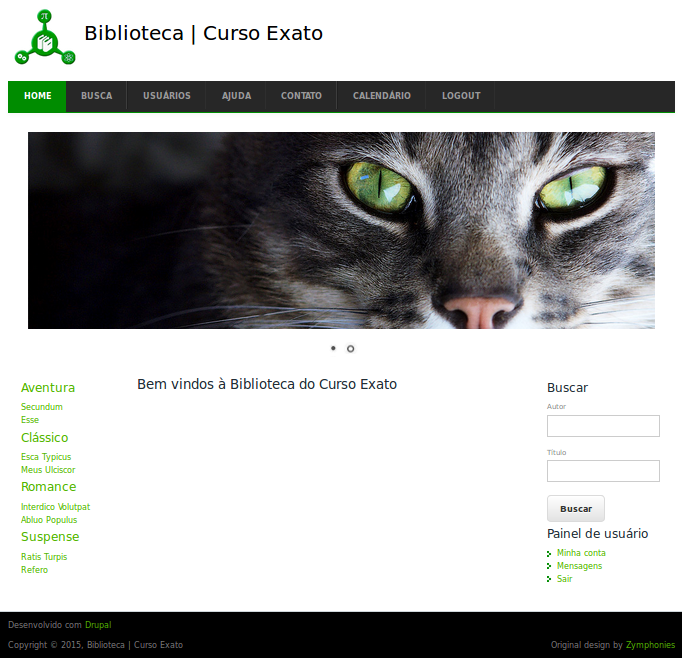
\includegraphics[width=140mm]{img/home-small.png}
\caption{Página inicial.\label{home}}
\end{figure}


\subsubsection{Criação de grupos de obras recomendadas por tema}\label{sssec:srecommended}
Foram definidos pelos membros do Curso Exato quatro temas - Aventura, Clássico, Romance e Suspense - para agrupar obras recomendadas na página inicial, visando facilitar a escolha dos livros aos usuários, principalmente àqueles que não possuem o hábito da leitura. Este agrupamento é feito em listas - uma para cada tema -, nas quais são exibidas até cinco publicações que atendam às seguintes condições: pertençam ao tema correpondente da lista e possuam o indicador de recomendação ativado. Caso existam seis ou mais publicações marcadas como recomendadas para um mesmo tema, apenas as cinco mais recentes (por data de inclusão no sistema) serão exibidas.

A Figura \ref{recommended} ilustra a listagem de temas na barra lateral esquerda da página inicial.

\begin{figure}[pbth!]
\centering
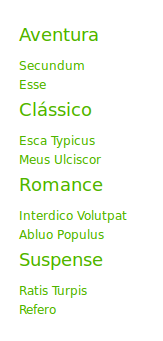
\includegraphics[width=30mm]{img/leftsidebar-close.png}
\caption{Obras recomendadas por tema.\label{recommended}}
\end{figure}

\subsubsection{Desenvolvimento do módulo \textit{Drupal} para geração de números de chamada}\label{sssec:chamada}

Foi desenvolvido e instalado um módulo \textit{Drupal} para a geração de números de chamada no momento da criação de uma página de publicação. Sua finalidade é facilitar o trabalho dos bibliotecários.

Houve uma sobrecarga de tempo considerável nesta tarefa devido a uma falha no formato de código de tombo e do número de chamada adotado inicialmente na biblioteca. Não havia uma distinção clara entre o \textit{número de chamada} - concatenação de letras e números, relacionada à \textit{publicação}, para auxiliar principalmente a manutenção da biblioteca física - e o \textit{código de tombo} - identificador único, relacionado ao \textit{exemplar}, para controle de transações no sistema. A falta de clareza sobre essa diferença, aliada à crença de que o tamanho reduzido do acervo não justificaria a criação de códigos mais elaborados, levou à falsa suposição de que um modelo de identificador unificado (isto é, uma combinação entre número de chamada e código de tombo) seria suficiente para gerenciar a biblioteca do Curso Exato. Nela, os exemplares de obras de mesmo título e autor recebiam um valor incremental, por ordem de cadastro na biblioteca. A Figura \ref{tombo-antigo} ilustra uma situação de cadastro de três exemplares do livro Vidas secas, de Graciliano Ramos.

\begin{figure}[pbth!]
\centering
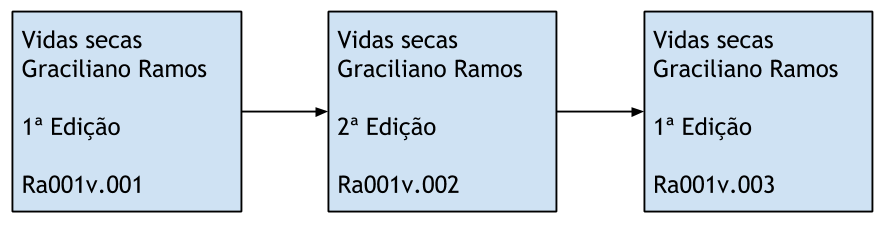
\includegraphics[width=120mm]{img/tombo-antigo.png}
\caption{Ilustração do modelo antigo de cadastro de exemplares da mesma obra.\label{tombo-antigo}}
\end{figure}

No entanto, percebeu-se durante o desenvolvimento do módulo que esta abordagem seria problemática por não dar ao aluno a escolha de qual edição da obra reservar. Além disso, a abordagem anterior pode complicar a organização das obras na estante. No exemplo da Figura \ref{tombo-antigo}, o bibliotecário teria a falsa impressão de que existe uma relação de ordem entre os exemplares, devido à indexação final do código. Entretanto, é mais útil manter o acervo agrupado por edições ou volume da obra, e não ordenado por este código.

A fim de se corrigir os problemas encontrados, duas ações foram executadas. A primeira ação foi redefinir os critérios de unicidade de uma publicação. Agora, a partir de um conjunto mais amplo de características de uma obra, um \textit{número de chamada} é criado para cada publicação, e cada exemplar pertencente a uma publicação recebe um \textit{código de tombo} diferente. A nova regra de unicidade de uma obra inclui, a editora, o ano de publicação, e edição e o volume, além de título e nome do autor, que já eram considerados. A segunda ação foi separar por completo o \textit{número de chamada} e o \textit{código de tombo}, e não mais apresentá-lo na forma concatenada na lombada do livro. O formato do número de chamada continuou sendo o mesmo (duas letras do sobrenome do autor, três dígitos e uma letra do título da obra). O código de tombo continua sendo representado por número inteiro, mas é gerado de forma diferente. Na plataforma \textit{Drupal}, cada página de conteúdo criada recebe um identificador. No caso específico da página em questão representar um exemplar, este identificador é também utilizado como código de tombo. Uma vez que o \textit{Drupal} provê um identificador de página único e autoincrementado, tem-se a garantia de não haver conflito entre códigos de tombo. A Figura \ref{tombo-novo} e a Tabela \ref{tabela-tombo-novo} ilustram a mesma situação de cadastro utilizada no exemplo anterior.

\begin{figure}[pbth!]
\centering
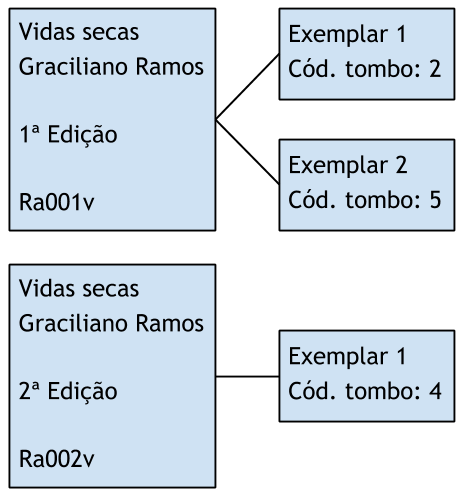
\includegraphics[width=60mm]{img/tombo-novo.png}
\caption{Ilustração do modelo novo de cadastro de exemplares da mesma obra.\label{tombo-novo}}
\end{figure}

\begin{table}[hc]
\centering
\caption{Conteúdos gerados na plataforma \textit{Drupal} seguindo a Figura \ref{tombo-novo}.\label{tabela-tombo-novo}}
\begin{tabular}{llll}
\hline
\# página & Título                                & Tipo       & Data de criação  \\ \hline
5         & Exemplar 2 de Vidas secas (1ª edição) & Exemplar   & 2015/10/31 12:58 \\ \hline
4         & Exemplar 1 de Vidas secas (2ª edição) & Exemplar   & 2015/10/30 10:16 \\ \hline
3         & Vidas secas (2ª edição)               & Publicação & 2015/10/30 10:16 \\ \hline
2         & Exemplar 1 de Vidas secas (1ª edição) & Exemplar   & 2015/10/28 18:38 \\ \hline
1         & Vidas secas (1ª edição)               & Publicação & 2015/10/28 18:38 \\ \hline
\end{tabular}
\end{table}


\subsubsection{Adaptação de ferramenta para importação em lote de publicações}
Por meio do menu administrativo, os administradores da biblioteca podem cadastrar uma publicação e seus exemplares no sistema, manualmente. Porém, foi discutido entre os alunos desenvolvedores que este método de inserção manual seria demasiadamente custoso para massas de dados de tamanho considerável. Para minimizar este problema, idealizou-se a criação de um módulo capaz de gerar automaticamente tanto as páginas das obras quanto as dos múltiplos exemplares de cada uma delas (se houver). Para a construção deste, tomou-se como base o módulo \textit{Feeds}, capaz de importar \textit{feeds RSS} ou arquivos CSV em conteúdo \textit{Drupal}.

Apesar de não estar incluída no escopo original do projeto, esta ideia foi colocada em prática para facilitar a inclusão do acervo original e, porventura, de livros arrecadados em campanhas realizadas pelo Curso Exato.

Esta funcionalidade foi iniciada neste ciclo e finalizada no segundo. No primeiro ciclo, o módulo já era capaz de ler o arquivo CSV e importar as obras, mas ainda não criava os exemplares.

\subsection{Segundo ciclo de desenvolvimento}
Este ciclo, assim como o primeiro, iniciou-se após reunião com os supervisores do projeto. Nesta, questionou-se o motivo de se utilizar uma propriedade do \textit{Drupal} como código de tombo. A atribuição de identificadores únicos de páginas geradas pela plataforma a itens não virtuais causaria complicações no cenário de migração do sistema para outra plataforma, pois o mecanismo de geração de códigos de tombo não estaria mais disponível. Discutiu-se, entretanto, que esta possibilidade era consideravelmente remota e, uma vez validado o fato junto aos responsáveis pela biblioteca do Curso Exato, decidiu-se que tal abordagem seria mantida. Desta forma, cada publicação conteria uma referência (lista de identificadores) para as páginas dos seus exemplares e, no momento em que suas páginas são processadas para exibição no navegador, o conteúdo dos exemplares poderia ser carregado rapidamente. Estas informações podem ser utilizadas para que se determine, dentre os exemplares de uma publicação, quais e quantos estão disponíveis para reserva, por exemplo.

%% Talvez substituir "alunos desenvolvedores" por "nós", com aprovação da Chris para isso.
Algumas funções providas pela plataforma e necessárias para a implementação de novas funcionalidades para este ciclo eram desconhecidas dos alunos desenvolvedores. Desta forma, houve necessidade de um estudo específico ao longo deste período, especialmente para a elaboração do mecanismo de registro de transações dos livros da biblioteca e para a conclusão da ferramenta de importação em lotes. Devido a isso, algumas tarefas, inicialmente previstas para este ciclo, foram concluídas no seguinte.

A seguir, são descritas as atividades realizadas durante o segundo ciclo de desenvolvimento.


\subsubsection{Finalização da ferramenta para importação em lote de publicações}

Durante a segunda semana do ciclo foi concluída a ferramenta de importação em lotes. Devido à alta ocorrência de vírgulas nos textos dos campos a serem registrados, definiu-se que o separador padrão dos arquivos CSV de entrada será o ponto e vírgula (;) e que cada linha deve conter as informações descritas na Tabela \ref{csv}, que descreve os atributos do arquivo solicitado na importação.

\begin{table}[hc]
\centering
\caption{Atributos requeridos no arquivo CSV.\label{csv}}
\begin{tabular}{ll}
\hline
\textit{title} & Título da publicação \\
\textit{author} & Nome do autor (formato: SOBRENOME, Nome) \\
\textit{publisher} & Editora \\
\textit{year} & Ano de publicação \\
\textit{edition} & Edição \\
\textit{volume} & Volume \\
\textit{category} & Categoria (Luso-brasileira, Estrangeira, Infanto-juvenil ou Outros) \\
\textit{ncopy} & Número de exemplares a serem inseridos \\
\textit{collection} & Coleção \\
\textit{recommended} & Variável binária indicando se a publicação deve ser colocada \\
 & em destaque na seção recomendados (1 = recomendado) \\
\textit{state} & Estado de publicação \\
\textit{body} & Resumo da obra \\
\textit{theme} & Tema principal (Aventura, Clássico, Romance, Suspense) \\
\textit{translator} & Tradutor \\
\hline
\end{tabular}
\end{table}

Houve certa dificuldade no registro das referências cruzadas entre publicações e seus exemplares devido ao modo como o \textit{Drupal} trata a criação paralela de páginas de conteúdo. O importador de arquivos CSV do módulo \textit{Feeds} cria uma requisição para a criação de uma nova página de conteúdo a cada linha lida do arquivo. Em nossa abordagem inicial, esta página a ser criada era de \textit{publicação} e, assim que esta era registrada no sistema, novas requisições para a criação das páginas dos \textit{exemplares} relacionados eram lançadas. Tais páginas eram, então, criadas, recebendo um identificador único e uma referência à página da publicação a qual pertencem e, finalmente, a página da publicação era atualizada com os identificadores de seus exemplares recém-cadastrados, resultando na referência cruzada entre eles. No caso em que a linha do arquivo CSV se referisse a uma publicação já registrada no sistema (segundo os critérios de unicidade discutidos na seção \ref{sssec:chamada}, foi proposto que a requisição inicial para a criação da página de publicação fosse ignorada, e que apenas os exemplares pudessem ser criados. Contudo, descobriu-se não ser possível cancelar a requisição inicial sem comprometer a sequência de criações e atualizações de páginas. A solução encontrada foi declarar um novo tipo de conteúdo, que armazena os dados obtidos do arquivo CSV e intermedia a criação de publicações e exemplares - este foi nomeado \textit{Container}. Assim que um conteúdo do tipo \textit{Container} é registrado, o sistema verifica se a publicação cujos dados ele armazena já existe na base de dados. Caso ela seja encontrada, seus exemplares são cadastrados e sua página é atualizada com as referências deles; caso contrário, segue-se o fluxo de criação proposto anteriormente.

\subsubsection{Implementação de módulo para registro dos períodos de funcionamento da biblioteca}
Para a fácil manutenção das datas de funcionamento da biblioteca, foi instalado no sistema o módulo \textit{Availability Calendar}. Apesar deste ser voltado para sistemas de alocação e de reservas (em hotéis, por exemplo), verificou-se que ele fornece visuais aos administradores para que estes configurem possíveis datas para retirada de empréstimos e realização de devoluções. Com este módulo foi possível criar uma página na qual são exibidos, em forma de calendário, o mês atual e os doze próximos, atribuindo uma cor para cada célula, referente ao estado previsto da biblioteca naquela data. Definiu-se três estados possíveis: \textit{aberta}, \textit{fechada} e \textit{férias}.

O estado \textit{aberta} indica um dia em que a biblioteca do Curso Exato estará em funcionamento, logo, o aluno pode tomar emprestado seus exemplares reservados ou devolvê-los. A célula é exibida com um fundo verde. \textit{Fechada} indica que não haverá atividade da biblioteca naquela data (geralmente sextas-feiras, finais de semana, feriados letivos ou quaisquer dias nos quais não será possível a um voluntário se responsabilizar pela atividade). A célula é exibida com um fundo avermelhado. Por fim, \textit{férias} indica recesso. A célula é exibida com um fundo azul. Além do usuário não poder retirar empréstimos ou devolver exemplares neste período, qualquer prazo de devolução que for previsto para terminar durante o período de férias será reduzido para o último dia com o estado \textit{aberta}.

É importante notar que os prazos de funcionamento da biblioteca não necessariamente seguem o calendário letivo do Curso Exato. Na verdade, é recomendado que os administradores configurem os últimos dias letivos antes dos recessos do projeto de extensão como \textit{fechada}, para que se evitem problemas com devoluções em atraso.

\subsubsection{Implementação do fluxo básico de reserva, empréstimo, renovação e devolução de uma obra} \label{sssec:stransaction}
Na reunião de planejamento deste ciclo foi elaborado um diagrama simplificado de máquina de estados, para a representação do fluxo de empréstimo de um exemplar, apresentado na Figura \ref{workflow}. Os círculos referem-se aos possíveis estados de uma publicação durante o fluxo, \textit{disponível}, \textit{reservado}, \textit{emprestado}, \textit{em atraso} e \textit{extraviado}; as setas indicam as ações que levam à transição entre eles, sendo elas: \textit{criar exemplar}, \textit{reservar}, \textit{confirmar empréstimo}, \textit{cancelar reserva}, \textit{renovar}, \textit{notificar atraso}, \textit{confirmar devolução}, \textit{declarar perda} e \textit{recuperar exemplar}.

\begin{figure}[pbth!]
\centering
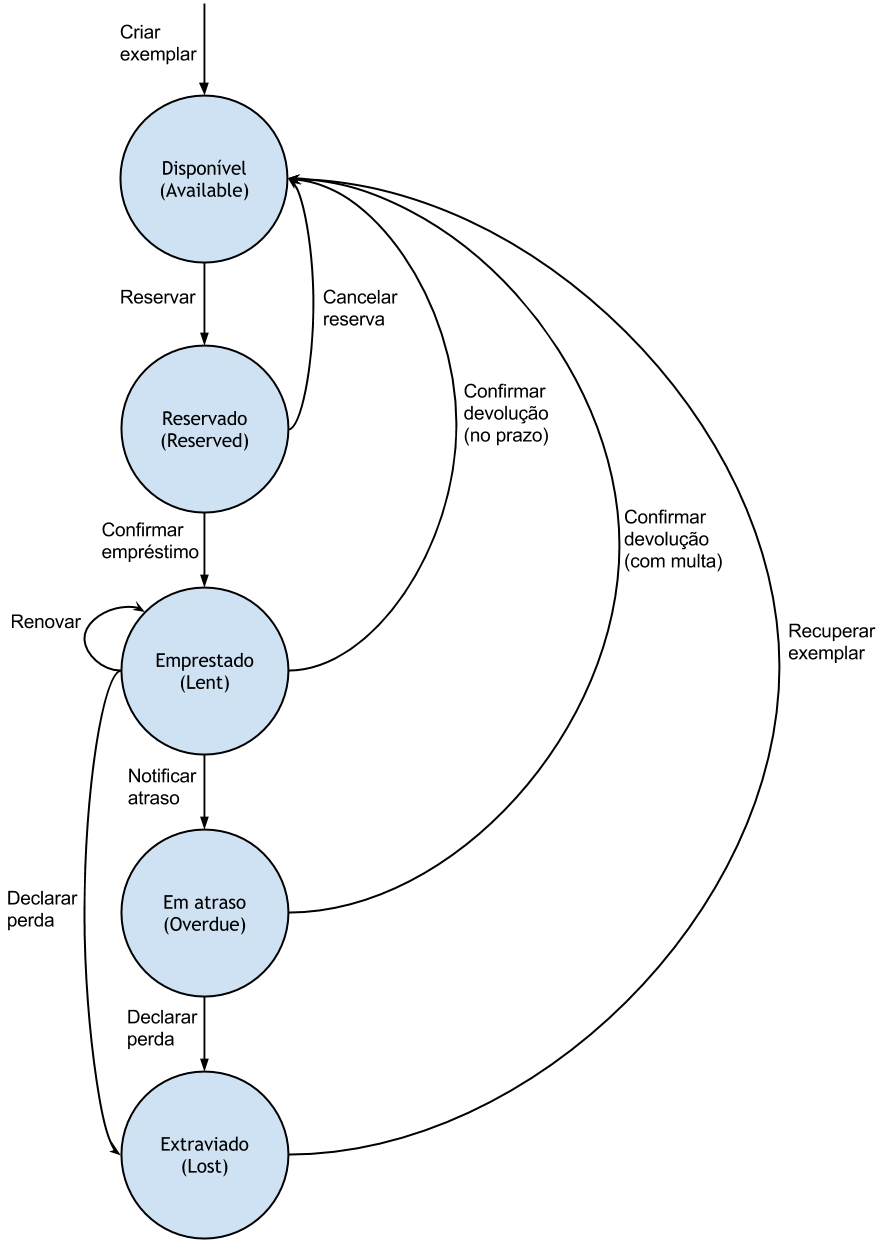
\includegraphics[width=140mm]{img/workflow.png}
\caption{Diagrama de máquina de estados de um exemplar durante o fluxo de empréstimo.\label{workflow}}
\end{figure}

Um exemplar é dito \textit{disponível} quando encontra-se disponível na biblioteca para reserva; \textit{reservado}, quando há uma solicitação de reserva por este exemplar a ser atendida; \textit{emprestado}, se o exemplar está em posse de algum usuário da biblioteca e o prazo de vencimento do empréstimo ainda não expirou; \textit{em atraso}, se o exemplar está em posse de algum usuário da biblioteca e deve ser devolvido, pois o prazo para devolução não foi respeitado; e \textit{extraviado}, se o exemplar foi perdido durante o fluxo de empréstimo.

Com relação às ações permitidas para cada classe de usuários, os administradores do sistema podem (a) \textit{criar exemplares} declarando a chegada de novos exemplares à biblioteca, inserindo-os no sistema individualmente ou pela ferramenta de importação em lotes; e os usuários autenticados no sistema podem (b) \textit{reservar} algum exemplar de publicações de seu interesse, clicando no botão ‘Reservar Livro’ na página da publicação. Esta ação só pode ser realizada por usuários que tenham dois empréstimos correntes ou menos, e que não tenham pendências com a biblioteca (ver Seção \ref{sssec:overdue_or_lost} para mais detalhes sobre fluxos alternativos).

Os administradores devem (c) \textit{confirmar o empréstimo} quando um exemplar é emprestado ao usuário que o reservou previamente e neste momento é calculado o prazo para devolução do exemplar (duas semanas após a data de confirmação). O usuário que solicitou uma reserva pode, sem sofrer penalidades, (d) \textit{cancelá-la}, sendo esta função também disponível para os administradores, quando houver um motivo específico e justificável.

Os administradores e o usuário em posse de um exemplar podem optar pela (e) \textit{renovação do empréstimo}, prolongando o prazo de devolução para uma semana após a data da renovação. Esta ação pode ser realizada no máximo duas vezes por empréstimo corrente e apenas se a data de vencimento do empréstimo estiver dentro do prazo de sete ou menos dias a partir da data da renovação. Quando um exemplar não é devolvido dentro do prazo previsto, o sistema automaticamente (f) \textit{notifica} o usuário envolvido e os administradores sobre o atraso e altera o estado do exemplar para \textit{em atraso}. Isto acarreta a aplicação de uma penalidade ao usuário (ver Seção \ref{sssec:overdue_or_lost}).

Após a devolução de um exemplar, os administradores devem \textit{confirmar o retorno} deste à biblioteca, encerrando o empréstimo. Se o estado que origina esta ação for \textit{emprestado}, a devolução foi (g) no prazo e não haverá nenhuma implicação ao usuário; se for \textit{em atraso}, o usuário será penalizado (h) com multa (vide Seção \ref{sssec:overdue_or_lost}). Os administradores e o usuário que tomou um exemplar emprestado podem (i) \textit{registrar o extravio} deste, o que leva à interrupção do empréstimo e dispara uma notificação aos administradores de que aquela cópia do livro dificilmente retornará à biblioteca. Esta ação acarreta uma penalização mais severa ao usuário (também descrita na Seção \ref{sssec:overdue_or_lost}). No caso de um exemplar previamente declarado como extraviado ser (j) \textit{recuperado}, administradores devem registrar seu retorno ao acervo. É importante ressaltar que esta ação não equivale à reposição de um exemplar extraviado por outra cópia da mesma publicação: para isto, a ação ‘Criar exemplar’ deve ser executada.

Foi definido também o conceito de transação: uma entidade para registro de cada passo do fluxo de empréstimo, desde a reserva até a devolução - cobrindo também os cenários alternativos. Definiu-se que uma transação envolvendo um exemplar é iniciada (criada no estado \textit{aberta}) no momento da sua reserva e se encerra ao atingir o estado \textit{cancelada} (quando a reserva é cancelada) ou \textit{encerrada} (quando o livro é devolvido ou recuperado após o extravio). O extravio é declarado pela mudança de estado da transação para \textit{exemplar perdido}. A tabela do banco de dados foi planejada para o armazenamento de transações, como na Tabela \ref{transactions-table}.


\begin{table}[hc]
\centering
\caption{Colunas da tabela de transações.\label{transactions-table}}
\begin{tabular}{ll}
\hline
Nome da coluna & Informação armazenada \\
\hline
\textit{id}                        & {Identificador único da transação} \\
\hline
\textit{last\_edit\_date}        & {Última data de modificação da transação} \\
\hline
\textit{status}                    & Estado da transação:\\
&                                1 - Aberta (Ongoing)\\
&                                2 - Cancelada (Canceled)\\
&                                3 - Encerrada (Done)\\
&                                4 - Exemplar perdido (Lost copy) \\
\hline
\textit{user\_id}                & {Identificador único do usuário que iniciou a transação} \\
\hline
\textit{pub\_id}                & {Identificador único da publicação envolvida} \\
\hline
\textit{copy\_id}                & {Identificador único do exemplar envolvido} \\
\hline
\textit{copy\_status}            & Estado da publicação\\
&                                (como definidos no diagrama de máquina de estados, numerados de 1 a 5) \\
\hline
\textit{renewals}                & {Número de renovações} \\
\hline
\textit{reservation\_date}        & {Data da solicitação da reserva} \\
\hline
\textit{loan\_date}                & {Data da confirmação do empréstimo} \\
\hline
\textit{expected\_return\_date}    & {Data máxima para devolução do exemplar emprestado} \\
\hline
\textit{actual\_return\_date}        & {Data da confirmação de devolução do exemplar} \\
\hline
\end{tabular}
\end{table}

Com estas decisões, foi desenvolvido um módulo que insere tal tabela na base de dados do sistema (seguindo os padrões da API do \textit{Drupal}) e habilita dois pontos de exibição das transações no sistema: um painel na área administrativa para o monitoramento de todas e um bloco na área de usuário para acompanhamento daquelas com as quais esteve envolvido. Em particular, no bloco da página de usuário, este teria apenas permissão para cancelar suas reservas e renovar suas transações correntes. A Figura \ref{transactions} mostra a página administrativa que os usuários administradores terão acesso para controlar as transações da biblioteca.

\begin{figure}[pbth!]
\centering
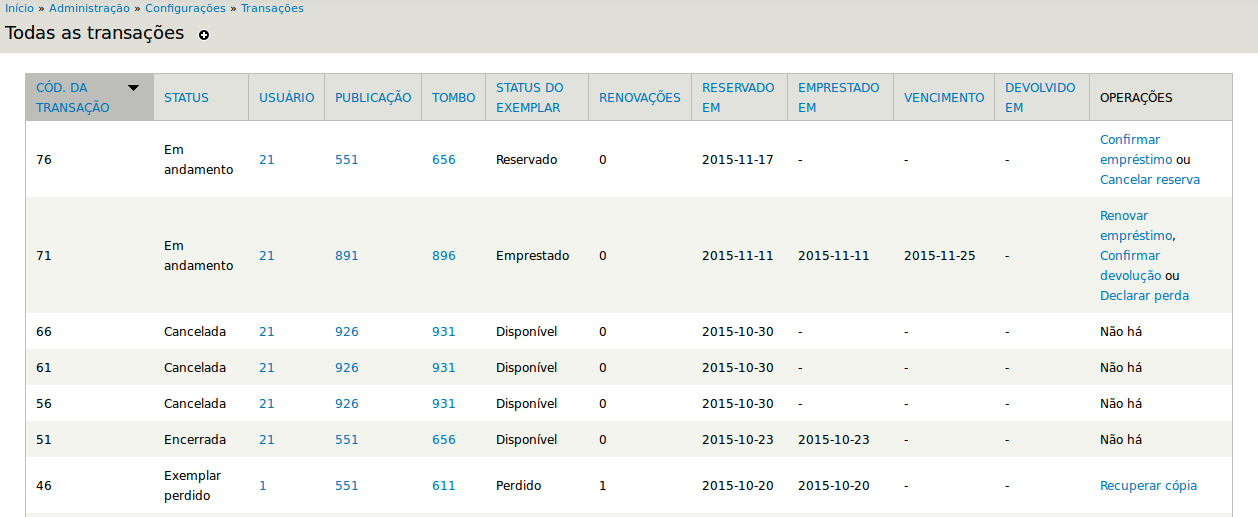
\includegraphics[width=140mm, trim={35mm 0 30mm 20mm}, clip]{img/transactions.png}
\caption{Painel de transações.\label{transactions}}
\end{figure}

Até o encerramento deste ciclo de desenvolvimento foi implementada boa parte dos passos do fluxo por parte do administrador. Os comportamentos restantes são a validação das datas de algumas ações em comparação com os dias de funcionamento da biblioteca e a exibição das transações envolvendo os usuários em suas páginas pessoais.

\subsubsection{Fluxo alternativo considerando atrasos ou extravio de algum exemplar}\label{sssec:overdue_or_lost}
Após reuniões com representantes do Curso Exato, foram coletadas algumas possibilidades de penalizações a serem aplicadas aos usuários que não respeitarem prazos de devolução de seus empréstimos ou àquelas que venham a perder algum exemplar emprestado:

\begin{enumerate}
\item Em caso de não devolução no prazo, o usuário perde o direito de reservar publicações ou de renovar empréstimos até que o usuário entregue a algum professor da área de Português do Exato uma resenha do livro lido, escrito à mão. Este prazo de multa seria similar ao aplicado por outras bibliotecas da Unicamp para alunos com exemplares em atraso, sendo ele proporcional à quantidade de publicações em atraso e à quantidade de dias de atraso.
\item Em caso de extravio de publicação emprestada, o usuário perde acesso ao sistema até que a cópia perdida seja ressarcida, ou que uma cópia de outra publicação de valor semelhante seja doada à biblioteca.
\end{enumerate}

Nas propostas acima, a condição de pendência do usuário seria registrada por duas variáveis binárias: uma para indicar multa por atraso e outra, por extravio. Ambas receberiam o valor $1$ caso as condições da aplicação das penalidades fossem detectadas - na confirmação da devolução no caso do atraso e na confirmação da perda no caso do extravio. Seus valores permaneceriam salvos até que algum administrador registrasse que a pendência foi resolvida.

\subsubsection{Envio e moderação de comentários nas páginas das publicações}

Foi habilitada a opção nativa do \textit{Drupal} que permite aos usuários autenticados enviarem comentários sobre as páginas de conteúdos existentes no sistema. Restringiu-se esta funcionalidade apenas a páginas de publicação.

Como solicitado pela coordenadora geral do Curso Exato, foi dada aos administradores a permissão para aprovar comentários antes que sejam publicados. Dessa forma, havendo necessidade de moderação, um administrador poderia advertir o usuário sobre o conteúdo impróprio do comentário enviado e impedir sua exibição aos demais visitantes do sistema.

\subsubsection{Revisão do controle de permissões}

Com o objetivo de garantir a integridade do sistema, buscou-se mitigar as possíveis brechas de segurança por comportamento indevido de usuários. Foram criadas contas de usuário para fins de teste - uma para cada classe de usuário definida na Seção \ref{ssec:tech} - e, acessando o sistema por meio delas, foi avaliado se usuários não autenticados possuíam permissão para acessar funcionalidades relacionadas a transações, e se usuários não administradores possuíam permissão para visualizar páginas de gerenciamento do sistema.

O núcleo do sistema \textit{Drupal} provê uma página administrativa para a configuração destas permissões. Dentre os testes realizados, verificou-se que os endereços administrativos disponíveis no próprio núcleo já estavam devidamente protegidos. Porém, em testes envolvendo endereços criados pelos módulos personalizados para este sistema, o resultado não foi o mesmo. Algumas ações não foram tratadas e a correção destas omissões foi alocada para o terceiro ciclo de desenvolvimento.

%%%
\subsection{Terceiro ciclo de desenvolvimento}

O terceiro ciclo de desenvolvimento teve seu início imediatamente após a reunião referente aos avanços do segundo ciclo com o supervisor Fábio. Como foi dito anteriormente, a este ciclo foram adicionadas algumas atividades extras, que não puderam ser concluídas no ciclo anterior. Todas as atividades propostas para finalização neste ciclo foram cumpridas, exceto a tradução total do sistema do inglês para o português brasileiro.

\subsubsection{Aplicação de penalidades devido ao fluxo alternativo}
    
Após discussão com os responsáveis pela biblioteca, optou-se pela simplificação do sistema de penalidades apresentado no ciclo anterior. Não há mais distinção entre os dois tipos de penalidade, então, basta uma única variável binária para registro da situação de um usuário. Esta tem seu valor ajustado para $1$ após qualquer operação em que se registre atraso na devolução ou perda de exemplares, e caberá aos bibliotecários realizar as cobranças correspondentes aos alunos punidos.
    
Certificou-se que o estado de penalidade impede o usuário de realizar novas reservas e renovações. Além disso, para que o usuário esteja ciente de sua penalização, uma mensagem de erro será exibida no sistema após a autenticação do usuário. 

\subsubsection{Finalização do painel de monitoramento de transações e desenvolvimento de mecanismo de proteção às mudanças de estado de transações}
    
Neste ciclo, foram concluídas as validações referentes às alterações de estado das transações. Porém, como as operações definidas para atualização das transações são ativadas via URLs específicas do sistema, foi percebido um problema, pois um usuário que conhecesse a ordem dos endereços acessados para registrar os passos do fluxo de empréstimo comum (da reserva até a devolução) poderia querer fazê-lo na ordem incorreta. Como solução, buscou-se garantir que os usuários não as ativem na ordem incorreta - acidental ou propositalmente, como mostra o exemplo a seguir: um bibliotecário pode reconhecer que os \textit{links} \textit{Confirmar empréstimo} e \textit{Confirmar devolução} do painel administrativo redirecionam o usuário a endereços do sistema que, ao serem acessados, completam as respectivas alterações de estado da transação. No entanto, caso ele acesse diretamente o endereço para confirmação de empréstimo, enviando como parâmetro um identificador de transação inválida - isto é, cujo exemplar não se encontre no estado \textit{Reservado} - o sistema não completará a ação e emitirá uma mensagem de erro.

Concluído este painel de monitoramento, foi elaborado um painel secundário para visualização apenas dos empréstimos cuja data de vencimento se encontre a sete dias ou menos a partir da data corrente. Este foi requisitado pelos administradores para facilitar o controle sobre as cobranças a serem feitas aos alunos. Assim, todos já estariam cientes de quais usuários possuem empréstimos com validade em data próxima logo no início da semana letiva do Curso Exato, podendo tomar providências - como notificá-los sobre a proximidade da data de devolução - antes que penalidades sejam aplicadas.

\begin{figure}[pbth!]
\centering
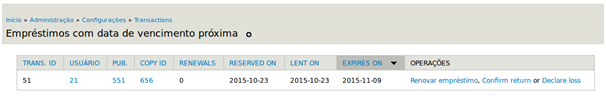
\includegraphics[width=150mm]{img/expiring-soon.png}
\caption{Empréstimos com data de vencimento próxima.\label{expiring-soon}}
\end{figure}

\subsubsection{Tela administrativa para controle de usuários}

Foi criado um terceiro painel administrativo, similar aos anteriores, para o monitoramento dos usuários que se encontram suspensos devido a pendências não resolvidas com a biblioteca. A motivação para a criação desta tela foi facilitar o controle das cobranças que devem ser feitas aos usuários quanto a atrasos ou perdas, e tornar mais prática a ação de desbloqueio de contas de usuário. Sem esta tela administrativa, seria necessário acessar cada página de usuário individualmente para efetuar múltiplos desbloqueios.

\begin{figure}[pbth!]
\centering
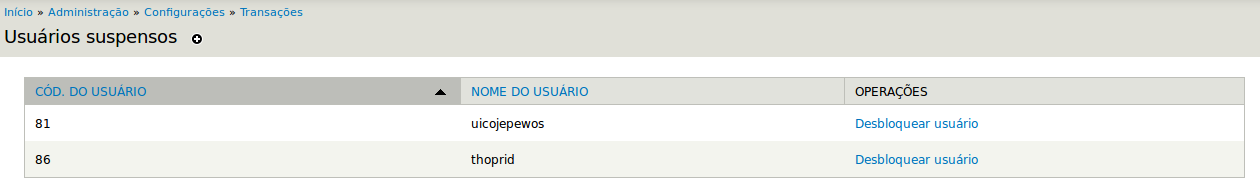
\includegraphics[width=120mm]{img/suspended-users.png}
\caption{Usuários suspensos.\label{suspended-users}}
\end{figure}

\subsubsection{Correção de \textit{bugs} referentes ao controle de permissões}
    
Durante o desenvolvimento das telas anteriores foram encontrados problemas no fluxo de empréstimo quando certas ações eram realizadas por usuários autenticados. Especificamente, notou-se que usuários com empréstimos correntes não possuíam permissão para renová-los em qualquer situação - embora o link referente a esta operação estivesse disponível na página do usuário - e que, em caso de erro em operações ativadas a partir da página de usuário comum, o usuário era redirecionado ao painel administrativo - causando um erro de acesso negado a todos os não administradores.

Após investigação, foram encontradas e corrigidas as falhas no código (\textit{bugs}) que provocaram este comportamento inesperado. A causa do problema consistiu na existência de cenários não previstos inicialmente, quanto ao fluxos de empréstimo e renovação, do ponto de vista dos usuários comuns.

\subsubsection{Preparação para implantação no servidor disponível para o Curso Exato}

O primeiro ponto levantado foi o local para a implantação do sistema, dadas algumas exigências e implicações por parte do Curso Exato. Após estudar as possibilidades e avaliar os pontos favoráveis e os contrários a cada opção, decidiu-se estabelecer o sistema no servidor de projetos discentes do Instituto de Computação (IC) da Unicamp, de forma a lançá-lo o mais breve possível. Tomada a decisão junto aos supervisores, os graduandos entraram em contato com a responsável pela Diretoria de Informática do IC para uma conversa inicial sobre a viabilidade de se hospedar o projeto naquele servidor. Durante esta reunião, foi acordado enviar uma breve descrição dos requisitos e das especificações técnicas sobre o que o sistema exigiria do servidor, para análise real da viabilidade desta implantação, e aguardar um posicionamento da Comissão Diretora de Informática do instituto.

De forma a não atrasar a implantação, os graduandos realizaram testes de exportação do sistema do ambiente de desenvolvimento (\textit{Acquia}) para outros locais, com o propósito de verificar a ocorrência de alguma dependência imprópria de módulos ou mesmo alguma dependência cíclica. Certificou-se que o sistema está em estado consistente e exportável como um pacote, por meio do módulo \textit{Features} do \textit{Drupal}. Este módulo permite o empacotamento de código, dependências, funções e variáveis de ambiente de uma instalação \textit{Drupal} em um arquivo comprimido, e a incorporação destes dados em uma outra instalação.

\subsubsection{Tradução da aplicação}

Na interface administrativa do \textit{Drupal}, existe uma seção que estima a quantidade e o percentual de termos traduzidos na aplicação. Por meio dela, verificou-se que aproximadamente vinte e cinco por cento dos termos utilizados na aplicação se encontravam sem tradução disponível para a Língua Portuguesa. Incluem-se no conjunto de termos não traduzidos as expressões e os rótulos definidos pelos graduandos nos módulos desenvolvidos para o funcionamento da biblioteca. A solução adotada foi utilizar o módulo \textit{Locale}, disponível no núcleo do \textit{Drupal}, para importar arquivos de traduções (extensão .po) no sistema. Este módulo busca automaticamente por traduções fornecidas por contribuidores da comunidade \textit{Drupal} disponibilizadas na página localize.drupal.org \cite{localize}; para termos não encontrados neste diretório, decidiu-se criar e importar manualmente um arquivo .po com sugestões de traduções.

Os alunos desenvolvedores se comprometeram a traduzir todas as expressões criadas para uso nos módulos desenvolvidos por eles. Para termos de outros módulos sem tradução fornecida pela comunidade \textit{Drupal}, houve um esforço pela inclusão de traduções para aqueles de maior ocorrência nas páginas do sistema; no entanto, por haver muitos e não haver um jeito direto de encontrar o contexto em que se localizam no sistema, não foi feita a tradução dos termos que não são exibidos diretamente aos usuários finais. Ressalta-se que a decisão por traduzir termos provenientes de módulos da comunidade em um arquivo .po, ao invés da submissão das traduções ao diretório público, foi motivada pelo longo tempo tomado até que haja uma aprovação das traduções enviadas por um moderador da comunidade \textit{Drupal}.

\section{Resultados} \label{sssec:improvements}
Utilizando a plataforma \textit{Drupal}, criou-se um sistema \textit{web} de gerenciamento de biblioteca com funcionalidades personalizadas para o contexto do Curso Exato. A aplicação não provê apenas requisitos essenciais de uma biblioteca, mas também inclui aspectos sociais, tais como: conversas individuais ou em grupo entre usuários, perfil pessoal, avaliação e resenha de uma publicação. Aprofundando os requisitos necessários para o sistema, os alunos desenvolvedores se depararam com um desafio. Houve certa discordância entre alguns membros do Curso Exato sobre políticas de auditoria de mensagens privadas e sobre a aplicação de penalidades em caso de atraso ou extravio de exemplares. Ainda assim, tais indecisões acarretaram apenas certo atraso até o alinhamento dos pontos questionados, mas não problemas de código durante o desenvolvimento, uma vez que tais questionamentos não fazem parte do fluxo do usuário. Pode-se afirmar, portanto, que o principal objetivo proposto neste trabalho foi concluído. 

Realizou-se uma apresentação do sistema a todos os futuros usuários, tanto alunos quanto professores voluntários do Curso Exato na ocasião do encerramento das atividades do projeto de extensão deste ano. Durante o evento foi possível notar que os presentes se mostraram satisfeitos, com uma reação particularmente positiva quanto às funcionalidades sociais. Considera-se a decisão pela inclusão destas uma escolha apropriada dos responsáveis pela biblioteca, apesar dos conflitos de opiniões que elas causaram.

Ao longo de todo o período de desenvolvimento foram levantadas diversas funcionalidades e melhorias que não foram implementadas devido ao tempo limitado, e por não estarem no escopo inicial do projeto. Uma das mais relevantes seria a alteração do fluxo de empréstimo para permitir a reserva de um exemplar enquanto este se encontra emprestado por outro usuário, tal como é possível nas bibliotecas da Unicamp. Pode-se destacar também processos de deleção lógica\footnote{Armazenamento de uma variável binária para indicar se houve uma requisição de remoção de um conteúdo; isto é, a aplicação não considera o conteúdo existente mas este continua armazenado no banco de dados.} de publicações ou exemplares do sistema, além de reaproveitamento de números de chamada. Reescrever o código para torná-lo mais modular também é uma tarefa necessária a longo prazo, para melhor manutenibilidade do sistema.

\section{Conclusão}
Ao longo deste projeto os alunos desenvolvedores puderam vivenciar o processo de desenvolvimento ágil com um time bastante reduzido. Isto permitiu avaliar vantagens e desvantagens de se adotar o \textit{Scrum} em contextos semelhantes. Considera-se como aspectos positivos de maior importância as entregas periódicas de versões funcionais do sistema e a realização de reuniões frequentes com os responsáveis pela biblioteca e com os supervisores do projeto - ações tomadas para manter o envolvimento dos indivíduos interessados no resultado final e assegurar a aceitação destes pelo o que estava sendo produzido. No entanto, questionou-se a adaptabilidade deste método para times reduzidos. A divisão de papéis não foi seguida durante todo o período de desenvolvimento devido a maior dificuldade de algumas tarefas, que exigiram o esforço de ambos os desenvolvedores. Além disso, as reuniões retrospectivas não foram realizadas com a frequência esperada porque não foram registrados muitos pontos de melhoria no processo de desenvolvimento a serem discutidas; dada a convivência praticamente diária entre os desenvolvedores, quaisquer sugestões de melhoramento foram discutidas e acatadas assim que idealizadas.

Destas observações, argumenta-se que metodologias ágeis diferentes poderiam ter sido mais apropriadas para este projeto. Avalia-se que a adoção do \textit{Kanban} \cite{kanban} ou do \textit{XP} (\textit{eXtreme Programming}) \cite{xp} poderia resultar em uma maior produtividade no processo de desenvolvimento. Ambos oferecem facilidades para a autogestão, são menos restritivas quanto aos papéis dos indivíduos no time desenvolvedor e dão menos ênfase na obrigatoriedade das reuniões - embora ainda valorizando os princípios do desenvolvimento ágil. Ainda assim, os alunos desenvolvedores se encontram satisfeitos com os resultados obtidos, e com a possibilidade dos alunos do Curso Exato terem acesso ao acervo da biblioteca do projeto \textit{on-line}.

Considera-se esta experiência gratificante por proporcionar situações reais enfrentadas por times de desenvolvimento, incluindo prazos reduzidos para entrega de funcionalidades, além de conflitos de interesses e níveis de entendimento entre os indivíduos envolvidos. Aprendeu-se muito sobre conceitos da Biblioteconomia e da gestão de projetos, além de haver um aprofundamento dos conhecimentos sobre a plataforma \textit{Drupal}, segurança da informação e usabilidade de interfaces humano-computador.

\pagebreak
\section*{Glossário}
\addcontentsline{toc}{section}{Glossário}
\begin{description}
\item[API (\textit{Application Programming Interface})] \hfill \\ Interface de programação de aplicações
\item[CMS (\textit{Content Management System})] \hfill \\ Sistema de gerenciamento de conteúdo
\item[Conteúdo \textit{Drupal}] \hfill \\ Página \textit{web} gerada pelo \textit{Drupal}, geralmente visível ao usuário final.
\item[CSV (\textit{Comma-separated values})] \hfill \\ Formato de arquivo contendo valores separados por vírgulas (ou delimitadores similares)
\item[\textit{Feed} RSS] \hfill \\ Agregador de conteúdos de páginas \textit{web} (\textit{Rich Site Summary})
\item[Tipo de conteúdo] \hfill \\ Conjunto de propriedades que devem ser contidas em páginas de mesmo tipo.
\item[URL (\textit{Unified Resource Locator})] \hfill \\ Endereço de recurso (i.e. arquivo, página, função, etc.) disponível em um sistema \textit{web}.
\end{description}

\pagebreak
\begin{thebibliography}{9}
\bibitem{cursoexato} Curso Exato.\\Disponível em: <http://www.preac.unicamp.br/cursoexato/>.\\Acesso em: 8 jul. 2015
\bibitem{drupal} Drupal - Open Source CMS.\\Disponível em: <https://www.drupal.org>.\\Acesso em: 5 set. 2015
\bibitem{manifesto} Manifesto for Agile Software Development.\\Disponível em: <http://www.agilemanifesto.org/>.\\Acesso em: 12 jul. 2015
\bibitem{scrum} Core Scrum | What is Scrum | Scrum Principles - Scrum Alliance.\\ Disponível em: <https://www.scrumalliance.org/why-scrum/core-scrum-values-roles>. \\Acesso em: 20 jul. 2015
\bibitem{requirements} System requirements.\\Disponível em: <https://www.drupal.org/requirements>.\\Acesso em: 5 set. 2015
\bibitem{dewey} Dewey Decimal Classification.\\Disponível em: <http://www.gutenberg.org/files/12513/12513-h/12513-h.htm>.\\Acesso em: 5 set. 2015
\bibitem{cutter} Cutter classification.\\Disponível em: <http://forbeslibrary.org/research/cutter-classification/>.\\Acesso em: 5 set. 2015
\bibitem{trello} Trello.\\Disponível em: <https://trello.com/>.\\Acesso em: 5 set. 2015
\bibitem{acquia} CMS, Commerce, Community | Drupal.\\Disponível em: <https://www.acquia.com/>.\\Acesso em: 5 set. 2015
\bibitem{localize} Portuguese, Brazil overview | Translations\\Disponível em: <https://localize.drupal.org/translate/languages/pt-br/>.\\Acesso em: 27 nov. 2015
\bibitem{kanban} A Brief Introduction to Kanban | The Agile Coach\\Disponível em: <https://www.atlassian.com/agile/kanban>.\\Acesso em: 30 nov. 2015
\bibitem{xp} TANIGUCHI, K.; CORREA, F.E. "Metodologias ágeis e a motivação de pessoas em projetos de desenvolvimento
de software: Aplicando práticas de SCRUM e XP para promover a motivação de equipes de projetos
de desenvolvimento de software", in \textit{Revista de Ciências Exatas e Tecnologia}. São Paulo, v. IV, n. 4, 2009.

\end{thebibliography}
\end{document}
